We used the data gathered in tables \ref{tab:energyresults} and \ref{tab:matrixresults} to extract the physical properties of the continuum harmonic oscillator.
For both the energy gap and the matrix elements, according to equations \ref{eqn:fullen} and \ref{eqn:fullmat}, we performed a linear fit $y = m a ^2+q$ to find
$\Delta\tilde{E} = 0.9998(5)$ and $\matb = 0.4998(3)$ as the interception with the $y$ axis. The results are in good agreement with the theoretical values of $1$ and $0.5$.

Figures \ref{fig:contenergy} and \ref{fig:contmatelem} report the continuum limit for $\DEt$ and $\matb$ respectively, while figures \ref{fig:enerzoom} and \ref{fig:matzoom}
show close-ups of the points near the origin.

We also performed a \textit{full fit} those same equations to recover the frequency $\omega$ and the mass $m$ of the oscillator.
The results were satisfactory for the fit on $\DEt$, which had $\omega$ and $A$ as parameters
\begin{align}
  \DEt = \omega - \frac{\omega^{3}}{A}a^{2},
\end{align}
while the results for $\matb$ were less good. The model we used was
\begin{align}
  \matb = \frac{1}{2m\w}- \frac{\omega}{16 m}a^{2}
\end{align}
with $\w$ and $m$ as the fit parameters. Their values differ
from the expected ones by $8$ and $9$ standard deviations, but the correlation matrix suggests a very large negative correlation
between the fit parameters, which is not present in the theory
\begin{align}
  \label{eqn:cov}
  \crr =
  \begin{pmatrix}
    1 & -0.999\\
    -0.999 & 1\\
  \end{pmatrix}.
\end{align}

The results are collected in tables \ref{tab:entab} and \ref{tab:mattab}.
\begin{table}[h!]
  \centering
\begin{tabular}{@{}cccl@{}}
\toprule
\multicolumn{3}{c}{Linear fit}                 &           \\ \midrule
                   & Theoretical & Obtained    & $\sigma_{\text{s}}$ \\
$\Delta \tilde{E}$ & $1$         & $0.9998(5)$ & $0.4$     \\
Reduced $\chi^2$   & \multicolumn{3}{c}{$1.58$}            \\ \midrule
\multicolumn{3}{c}{Full fit}                   &           \\ \midrule
                   & Theoretical & Obtained    & $\sigma_{\text{s}}$ \\
$\omega$           & $1$         & $0.9998(5)$ & $0.4$     \\
$A$                & $24$        & $26.9(1.5)$ & $1.9$     \\
Reduced $\chi^2$   & \multicolumn{3}{c}{$1.58$}            \\ \bottomrule
\end{tabular}
\caption{\label{tab:entab}Continuum energy gap, frequency and $A$ parameter. All the results are inside a $2\sigma$ neighbourhood of their theoretical value. All the fits were performed by Gnuplot.}
\end{table}

\begin{table}[h!]
  \centering
\begin{tabular}{@{}cccl@{}}
\toprule
\multicolumn{3}{c}{Linear fit}               &           \\ \midrule
                 & Theoretical & Obtained    & $\sigma_{s}$ \\
$\matb$          & $0.5$       & $0.4998(3)$ & $0.67$    \\
Reduced $\chi^2$ & \multicolumn{3}{c}{$3.5$}             \\ \midrule
\multicolumn{3}{c}{Full fit}                 &           \\ \midrule
                 & Theoretical & Obtained    & $\sigma_{s}$ \\
$\omega$         & $1$         & $0.92(1)$   & $8$       \\
$m$              & $1$         & $1.09(1)$   & $9$       \\
Reduced $\chi^2$ & \multicolumn{3}{c}{$3.5$}             \\ \bottomrule
\end{tabular}
\caption{\label{tab:mattab} Results for the matrix element. The continuum limit is satisfactory, while the full fit returns incompatible results. The parameters extracted from the full fit also present a very high negative correlation (covariance matrix \ref{eqn:cov}), which could impact
the result of the fit. All the fits were performed by Gnuplot.}
\end{table}
%\onecolumn
%%------------------------ TABLE --------------------
\begin{table}[h!]
  \centering
\begin{tabular}{ccccccccc}
\hline
\multirow{2}{*}{} & \multirow{2}{*}{$N$} & \multirow{2}{*}{$a$} & \multirow{2}{*}{$D_{bin}$} & \multirow{2}{*}{$N_{bin}$} & \multicolumn{2}{c}{$\Delta\tilde{E}$}                            & \multicolumn{2}{c}{$\matb$}                                      \\ \cline{6-9}
           &       &                      &                            &                            & \multicolumn{1}{l}{Theoretical} & \multicolumn{1}{l}{Obtained} & \multicolumn{1}{l}{Theoretical} & \multicolumn{1}{l}{Obtained} \\ \hline
$A1$       &   $64$    & $1$                  & $50$                       & $20000$                    & $0.9624$                          & $0.9634(17)$                    & $0.4472$                         & $0.4477(7)$                   \\
$A2$       &   $128$   & $0.5$                & $500$                      & $10000$                    & $0.9899$                          & $0.9887(13)$                    & $0.4851$                         & $0.4850(5)$                   \\
$A3$       &   $256$    & $0.25$               & $500$                      & $10000$                    & $0.9974$                          & $0.9970(11)$                    & $0.4961$                         & $0.4965(5)$                   \\
$A4$       &   $512$    & $0.125$              & $1000$                     & $2000$                     & $0.99935$                          & $1.0002(6)$                    & $0.4990$                         & $0.4991(3)$                   \\
$A5$      &    $1024$    & $0.0625$             & $3000$                     & $2000$                      & $0.9998$                           & $0.9993(5)$                    & $0.4998$                         & $0.4999(3)$                  \\ \hline
\end{tabular}
\caption{\label{tab:bestvals}Summary of the lattices considered and their best values obtained for $\DEt$ and $\matb$.}
\end{table}
\twocolumn


%------------- FIGURES ------------
\begin{figure}[H]
  \centering
  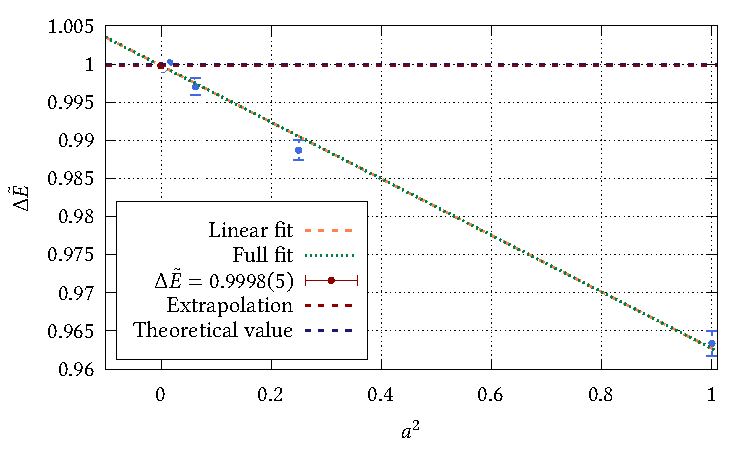
\includegraphics[width=\linewidth]{energy}
  \caption{\label{fig:contenergy}Energy gap continuum limit.}
\end{figure}
\begin{figure}[H]
  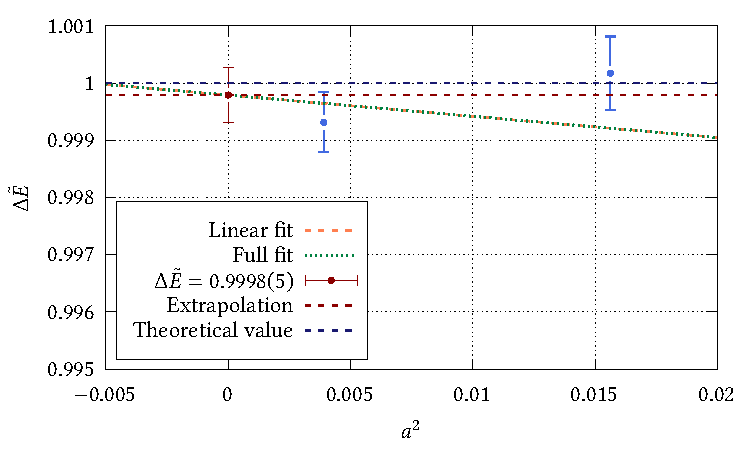
\includegraphics[width=\linewidth]{enerzoom}
  \caption{\label{fig:enerzoom}Close-up of the points next to the energy continuum limit.}
\end{figure}
\begin{figure}[H]
  \centering
  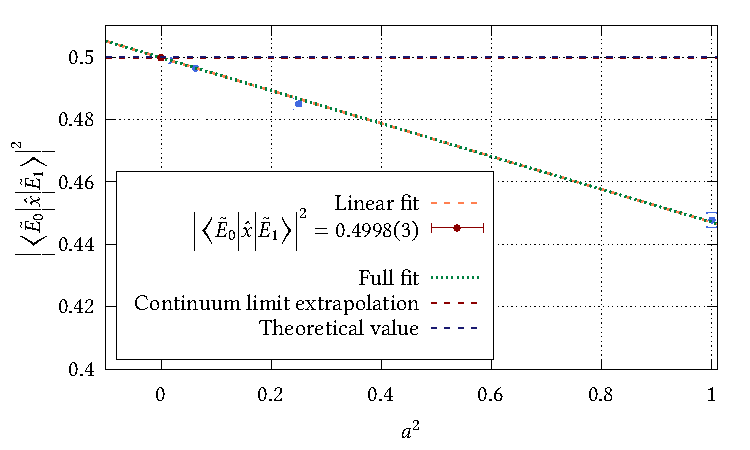
\includegraphics[width=\linewidth]{contmatelem}
  \caption{\label{fig:contmatelem}Matrix element continuum limit, error bars are doubled for visibility.}
\end{figure}
\begin{figure}[H]
  \centering
  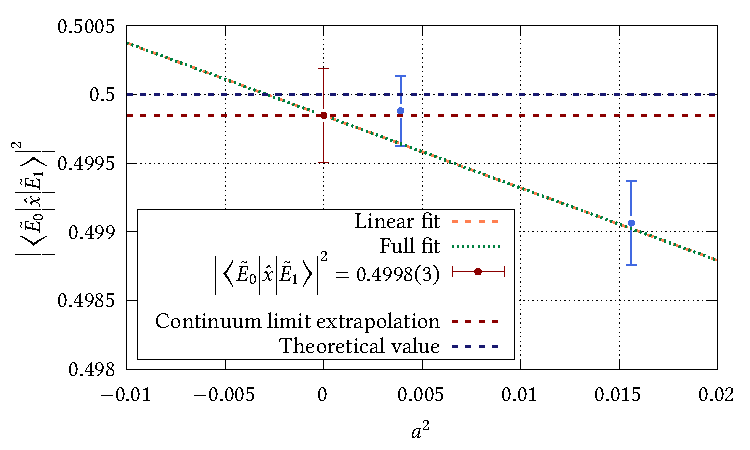
\includegraphics[width=\linewidth]{contmatelemtre}
  \caption{\label{fig:matzoom} Close-up of the points next to the matrix element continuum limit.}
\end{figure}
